\documentclass[]{report}

%\usepackage{helvet}
%\renewcommand{\familydefault}{\sfdefault}

\setcounter{secnumdepth}{0}
\usepackage[margin=1in]{geometry}
\usepackage{caption}
\usepackage{parskip}
\usepackage{float}
\usepackage{graphicx}
\usepackage{subcaption}
\usepackage[section]{placeins}
\newfloat{Equation}{H}{lop}
\usepackage[backend=biber, style=authoryear]{biblatex}
\addbibresource{./report.bib}

\title{
	The Relative Neuroplasticity of Artificial
	\linebreak
	and Biological Neural Network Configurations
}
\author{Oliver Balfour}

\date{%
	Alfred Deakin High School\\[2ex]%
	\today
}

\begin{document}
\maketitle

\begin{abstract}
	In this experiment the neuroplasticity of neural networks, both artificial and biological, was tested. Several configurations of computing machines, ranging from simple densely-layered feed-forward Multi-Layer Perceptrons (MLPs) and Artificial Neural Networks (ANNs) to more complex Recurrent Neural Networks (RNNs), were tested, using the human brain as a performance baseline, in order to gauge how far the field of Machine Learning has come in past decades both in terms of performance and neuroplasticity, measured in this investigation as the standard deviation of a model's error rate across a diverse range of problem domains. Each model was tested (with minor programmatic alterations to the input and output layers of each artificial model to account for differing input vector size) against several different classification and regression problems including but not limited to classifying handwritten digits and performing sentiment analysis on highly polarized movie reviews. The neuroplasticity of each model was then evaluated given the error rates of each model across all problems tested. It was found that the human brain is still overall the most neuroplastic model across the full set of problem domains, with RNNs close behind in most respects. The MLPs and ANNs performed well on classification problems, outperforming the RNNs and even the human brain in several problem domains, but entirely failed to converge on the sentiment analysis problem due to their inability to learn from sequential data samples of differing lengths.
\end{abstract}

\tableofcontents
\newpage

\section{Introduction}

The human brain is capable of rewiring itself throughout its lifetime (\cite{draganski2004neuroplasticity}). This feature, known as neuroplasticity, is the driving force behind the process of learning, and is present in a wide range of animals. It was first discovered in rats in 1964 (\cite{bennett1964chemical}), and the theory behind it has applications as far as artificial intelligence and machine learning. In this investigation, the extent to which various artificial and biological intelligent agents exhibit neuroplasticity is tested, by teaching the same models to perform very diverse tasks, compared to a baseline of the performance of the human brain.

The aim of this experiment is to determine how far behind in terms of neuroplasticity modern Artificial Neural Networks (ANNs) are when compared with the human brain. This is done by training the same artificial and biological neural network configurations to perform several different classification and regression tasks, and measuring the standard deviation of the error rates across each problem as a measure of neuroplasticity.

It is hypothesised that:
\begin{enumerate}
	\item The human brain will marginally surpass state-of-the-art ANN configurations in all problem domains, and will perform exceptionally well in all problem domains. (Refer to the method on page \pageref{itm:Method} for a full list of problems tested.)
	\item The Recurrent Neural Network (RNN) will perform well on all problems, most notably the sentiment analysis problem.
	\item The standard densely-layered feed-forward Artificial Neural Network (ANN) will perform acceptably on all problems except the sentiment analysis problem.
\end{enumerate}

\section{Literature Review}

Whilst there is plenty of literature on machine learning and neuroplasticity as distinct topics, there is very little pertaining directly to both. The only publicly available scientific paper relating to both merely documents a method for making an ANN neuroplastic (\cite{perwej12}), however its approach is in essence a synaptic pruning method for reducing overfitting in ANNs similar to the well-established method of neural network dropout, which randomly discards nodes from a neural network to reduce overfitting (\cite{dropout14}). The only other paper referring to both topics is behind an expensive journal paywall.

This experiment focuses on a neglected area within the field of machine learning: as artificial intelligence research is primarily focused on highly specialised cutting-edge techniques, investigation into the re-usability and adaptivity of neural networks has been left in the dust. Considering that an Artificial General Intelligence (AGI) requires an extremely neuroplastic brain to be capable of learning without requiring a considerable number of pretrained neural networks as sub-circuits for each individual task it is capable of performing, this investigation is important as a measure of the level of progress that the field of machine learning has achieved toward an AGI, not in terms of specialised narrow intelligence feats such as those of AIs designed solely to play games like Chess or Go at a highly competitive level, but in terms of how specialised narrow AI achievements can be generalised for the purpose of creating a neuroplastic general intelligence.

The techniques used to create neural networks in this experiment, however, are very well documented. The perceptron, an outdated artificial model of a neuron, was documented thoroughly by its creator (\cite{rosenblatt1958perceptron}), the multi-layer perceptron model, an improved model that featured hidden layers and the backpropagation algorithm was documented in a well established journal (\cite{rumelhart1986learning}); likewise, the original Support Vector Machine algorithm was well documented (\cite{vapnik1995support}). All of the neural network configurations used in this experiment rely on well-established methods that have been well-used in the field of AI research over the past few decades. Simple feed-forward backpropagated ANNs have been in wide use since the late 1980s, and RNNs were designed as an evolution on the simpler ANN and MLP structures, in their capability to create feature maps on sequential data.

\section{Background Information}

A neural network is essentially a simplified computer abstraction of a brain, with primitive and computationally inexpensive representations of the core functions of neurons in a biological brain. Neural networks are organised into layers, usually three or more, which contain a configurable amount of distinct artificial neurons. The first layer takes binary or floating-point input from the host computer program mapped to each input node in a consistent format (so as to make computation of concrete feature-maps possible), and the last returns binary output back to the host program. In feed-forward neural networks, the most common type of neural network, simulated signals pass forward through neurons one layer at a time without any form of recursion.

\begin{figure}[H]
	\centering
	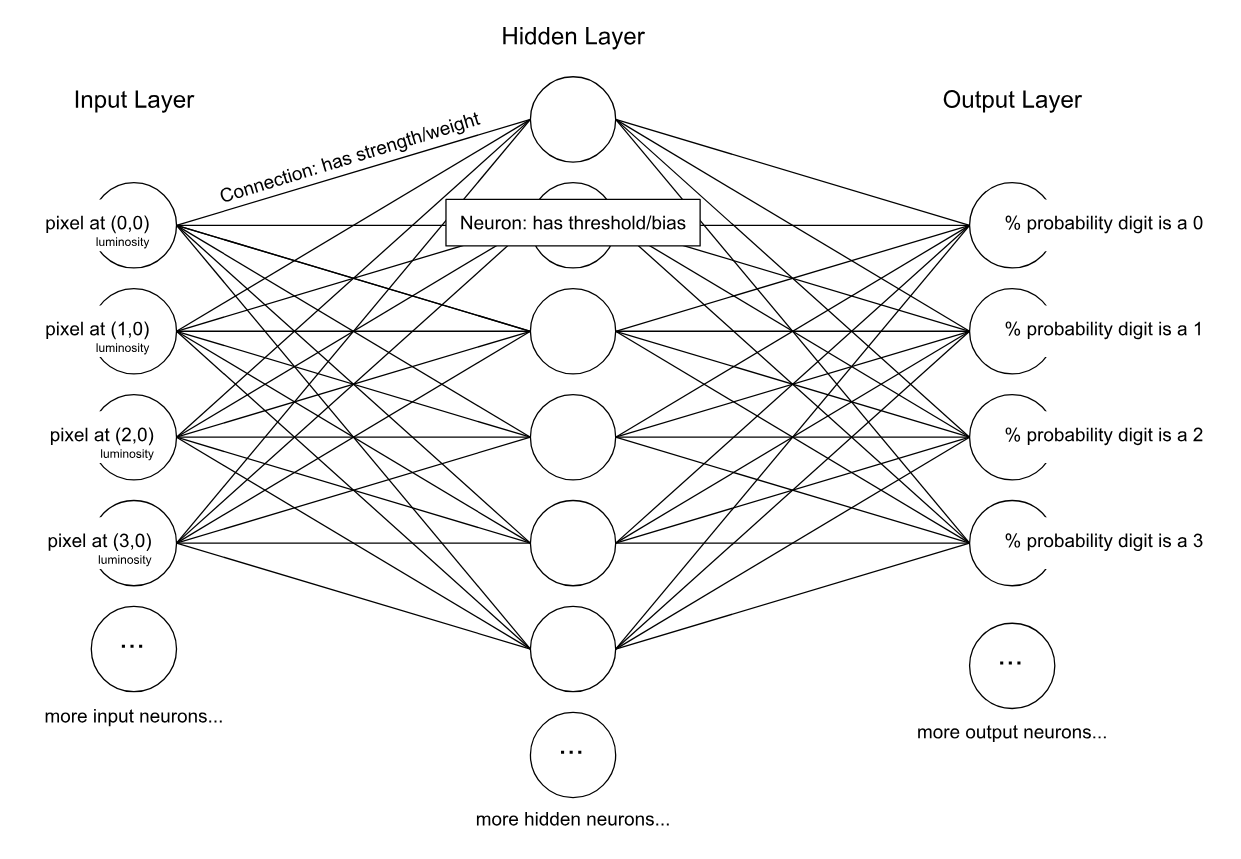
\includegraphics[width=0.8\textwidth]{network.png}
	\caption{Diagram of a feed-forward Artificial Neural Network trained to recognise digits.}
	\label{fig:network}
\end{figure}

A neuron is typically represented by a series of numbers: an activation threshold (bias), and a series of numbers representing the strengths of connections with neurons in the previous layer (weights). Given the outputs (activations) of the neurons in the previous layer (or given the input data from the host program in the case of the input layer), a neuron's output (activation) will equal the sum of all of the previous layer's neurons' activations multiplied by their respective connection weights, with the activation threshold of the neuron in question subsequently being subtracted. In a more traditional perceptron model, the output would be transformed such that if the intermediary activation value is positive it is transformed to a binary 1, or a binary 0 if it is negative; however more modern models using sigmoid or ReLU activation functions (see the glossary on page \pageref{sec:Glossary} for more information activation/learning functions) usually transform this value into a floating-point decimal between 0 and 1. Note that these calculations do not apply to the input layer, which simply takes the input from the host program and does not possess its own weights and biases.

\begin{Equation}
	\begin{equation}
		n_a = \left\{ \begin{array}{ll}
		0 & \mbox{if } \sum_{x \subset S} x_a x_w \leq n_b \\
		1 & \mbox{if } \sum_{x \subset S} x_a x_w > n_b
		\end{array}\right.
	\end{equation}
	\caption{Activation (output value) of a perceptron}
\end{Equation}

\begin{Equation}
	\begin{equation}
		n_a = \sigma(\sum_{x \subset S}(x_a x_w) - n_b)
	\end{equation}
	\caption{Activation of an artificial neuron, given an activation function $\sigma$}
\end{Equation}

In the above equations, \(S\) is the set of neurons from the previous layer, \(x_w\) is the weight (axon-dendrite connection strength) of the \emph{i}th neuron of \emph{S} with the neuron in question, and \(x_a\) denotes the activation; \(n\) is the neuron whose output is being calculated and \(n_b\) its bias, so the above formula is in essence adding all of the connection weights multiplied by their outputs, before subtracting the bias. The output is wrapped in a function to make the output smoother and more efficient in learning (for example by creating a sigmoid curve featuring a sharp slope toward the centre, which in training forces the weights and biases to either extreme), but the choice of learning function is an irrelevant implementation detail.

The weights and biases of each neuron and neuronal connection are optimised to serve a specific purpose through the process of training the neural network to perform a given task. Usually, these values will start as random numbers, and through a process known as Stochastic Gradient Descent (SGD) the values are slowly optimised until the model is sufficiently good at its task. In each iteration of the algorithm the trainable parameters of the model are randomly mutated, and the new model is tested for performance at the task. If the performance of the mutated model exceeds that of the original, the mutated model succeeds the original. This process is repeated millions of times until the performance starts to plateau. (Refer to the glossary on page \pageref{itm:SGD} for more information on SGD.) There are many applications for neural networks: A neural network may be trained to classify images (computer vision and optical character recognition), to estimate data such as house or stock prices given data about their respective markets, or even to control robots. This ability to excel in a wide range of problem domains is investigated in this report.

Nodes in neural networks are quite similar to their biological counterparts, in that they have an activation threshold (in biological neurons this threshold is a constant -55mV for all neurons, whereas in artificial neurons this is a unique number which is recursively optimised throughout the training process), take input from other neurons they have connections with (although artificial neurons have differing connection strengths and are connected to all nodes in the previous layer; biological neurons simply have binary connection strenghts --- they either are or are not connected), and produce one output which is used as an input by additional nodes in the network. The primary difference between neural networks and biological brains is that brains, even in small creatures such as rodents, have many orders of magnitude more neurons, and learning algorithms in biological networks are the fine-tuned result of billions of years of evolution.

\label{itm:Method}
\section{Method}

There are 20 artificial neural networks and 1 biological neural network tested in this experiment, against 4 different classification and regression problems, each in different problem domains. The neural network configurations are as follows:

\begin{enumerate}
	\item 8 different densely-layered feed-forward Multi-Layer Perceptrons (MLPs) using perceptrons instead of sigmoid-activated neurons (2 sets of 4 different models with differing hidden layer configurations, one set with dropout (\cite{dropout14}) and one without).
	\newline
	The 4 hidden layer configurations are:
	\begin{enumerate}
		\item 1 hidden layer with 32 neurons
		\item 1 hidden layer with 256 neurons
		\item 2 hidden layers with 256 neurons each
		\item 2 hidden layers with 512 neurons each
	\end{enumerate}
	All dropout-enabled models have the dropout percentage set to 20\% (so 20\% of neurons are randomly discarded throughout the learning process.)
	\item 8 standard densely-layered feed-forward sigmoid Artificial Neural Networks (ANNs), with hidden layer configurations identical to those of the MLPs above, aside from the nonbinary sigmoid activation function.
	\newline
	The sigmoid activation function used is defined as \(\sigma(x) = \frac{1}{1+e^{-x}}\)
	\item 4 Recurrent Neural Networks (RNNs), with 1 Long Short-Term Memory (LSTM) hidden layer containing 32 or 128 neurons. Two models have dropout, the others do not.
	\newline
	The recurrent neural networks use RMSprop (\cite{hinton2012neural}) instead of SGD as an optimisation algorithm, as it has been noted to perform better with RNNs.
	\item As a baseline for performance and neuroplasticity, several people were also used.
\end{enumerate}

It was decided that Convolutional Neural Networks (CNNs) should not be included in the experiment, as although they are a very popular type of neural network in image processing, they only work with multidimensional spatial or temporal data (their primary use-cases are in computer vision, optical character recognition, and audio analysis), and would require significant structural change to compute problems with non-temporal data (changing the convolutional layers between one and two dimensions at runtime). This means that they cannot feasibly compute linear regression or non-temporal classification functions without having their kernel layers configured to apply no transformation to the data (by having nil values for all kernel cells except the centre, which would have a 1, such that each kernel operation acts similarly to a cat program) or by being configured to operate in only one dimension.

Each of the above models is tested against the following classification and regression problems:

\begin{enumerate}
	\item Handwritten digit recognition (using the MNIST dataset\footnote{The MNIST dataset is available at: \texttt{http://yann.lecun.com/exdb/mnist/}})
	\item Iris flower classification (using Fisher's dataset\footnote{The iris dataset is available at: \texttt{http://archive.ics.uci.edu/ml/datasets/Iris}} (\cite{uciml2007}))
	\item Sentiment analysis (using the Large Movie Review Dataset\footnote{The movie review dataset is available at \texttt{http://ai.stanford.edu/~amaas/data/sentiment/}} (\cite{maas2011imdb}))
	\item Breast cancer diagnosis (using the University of Wisconsin dataset\footnote{The breast cancer diagnosis dataset is available at: \texttt{http://archive.ics.uci.edu/ml/datasets/Breast+Cancer+Wisconsin+(Diagnostic)}})
\end{enumerate}

The human brain was tested against each of the aforementioned problems, although due to the varying nature and medium in which the datasets above are presented (meaning different cortices of the human brain will be used for different problem domains) the human participants will have a significant advantage over their machine counterparts. The issue of human participants being able to use different cortices for different problems is unavoidable, as the only other alternative would be to present all data in an identical format, such as numerically, which would prove far too time consuming for participants.

The experiment was conducted in two phases for each combination of model (artificial or biological) and problem: the training phase, and the testing phase.

In the training phase, the artificial models were fed data along with the desired results from the respective datasets and left to their own devices, to implement their own optimisation algorithms. The participants were given the data similarly; however the data was printed and arranged in a more familiar format. (!)

In the testing phase, each model and participant was given data as in the previous stage, however the desired results were omitted, and the models and participants had to make predictions (or classifications, depending on the nature of the problem) based on inferences made from the training data. Note that participants were allowed to keep a copy of the training data for reference, due to memory and time limitations.

For each model-problem combination, the performance was measured as the accuracy of the model or participant in the testing phase. After testing a model against all of the problem domains, mean performance and neuroplasticity were calculated. Neuroplasticity was measured as the standard deviation of the performance/error rate (in calculating standard deviation only the distribution, and not the absolute values, were important, such that the standard deviation of the performance metrics and the error rates (inverse of the performance) were identical) of the model or participant across all of the problems tested (lower is better). In evaluating the overall performance of a model, both the mean performance and neuroplasticity metrics were considered as opposed to neuroplasticity alone, as a model which fails to converge on any problem domains and thus achieves a consistent 50\% accuracy could be said to be more neuroplastic than a model which performs excellently on some problems and acceptably on others when using standard deviation as a measure.

\begin{Equation}
	\begin{equation}
	\sqrt{\frac{((\sum_{i=0}^{|P|} P_i) - \bar{P})^2}{|P|}}
	\end{equation}
	\caption{Calculation of neuroplasticity, derived from the forumla for population standard deviation}
\end{Equation}

\section{Results}

The human error rates for the MNIST problem and breast cancer diagnosis were sourced from other literature; according to \cite{simard1993efficient}, the human MNIST accuracy averages at about 98.5\% (keeping in mind many of the samples are barely legible and written by high school students), and according to \cite{mangasarian1995breast} the accuracy of fine needle aspiration cytology (the method that ANNs in this investigation were trained to perform) as practiced by physicians averages at 82\%.

\textit{Note: in the following charts, model names are abbreviated such that a Multi-Layer Perceptron (MLP) with 2 hidden layers filled with 256 neurons and with dropout is denoted as \textit{MLP 256D,256D}, and without dropout as \textit{MLP 256,256}.}

\begin{figure}[H]
	\centering
	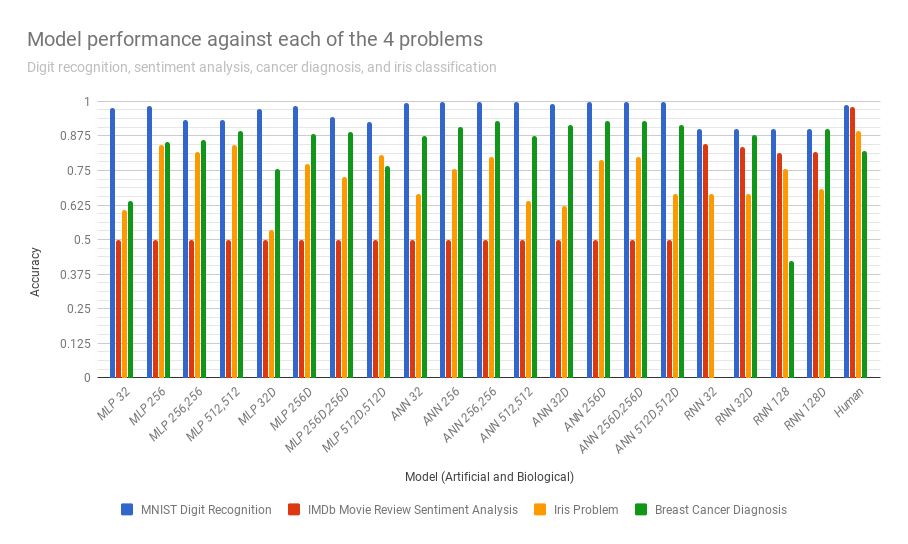
\includegraphics[width=\linewidth]{chart.png}
	\label{fig:chart0}
\end{figure}

\begin{figure}[H]
	\centering
	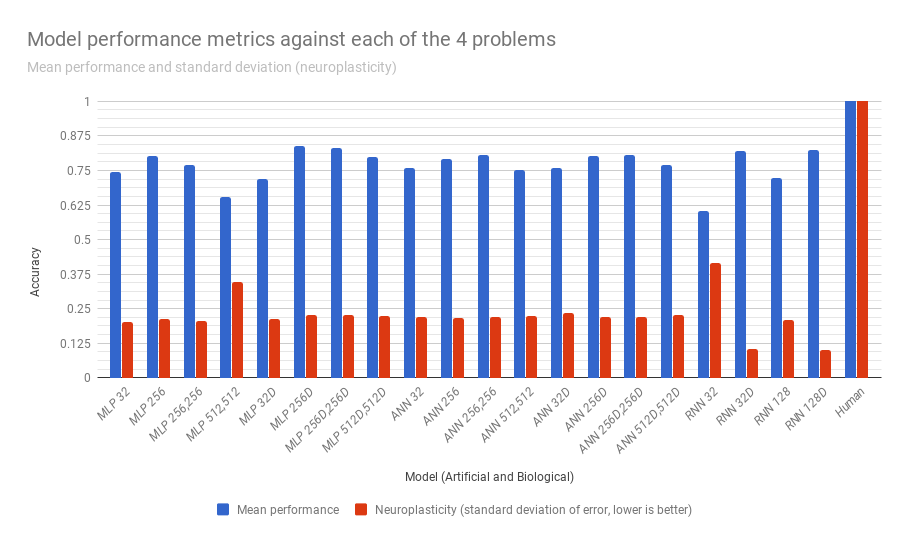
\includegraphics[width=\linewidth]{chart1.png}
	\label{fig:chart1}
\end{figure}

\begin{figure}[H]
	\centering
	\begin{subfigure}[b]{0.45\textwidth}
		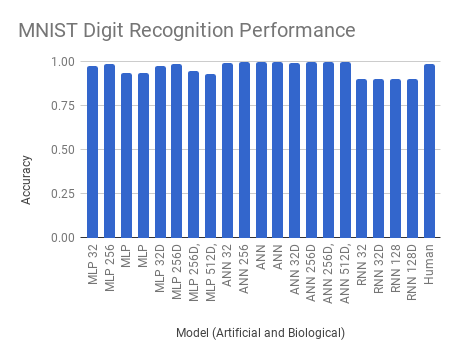
\includegraphics[width=\textwidth]{chart2.png}
	\end{subfigure}
	~
	\begin{subfigure}[b]{0.45\textwidth}
		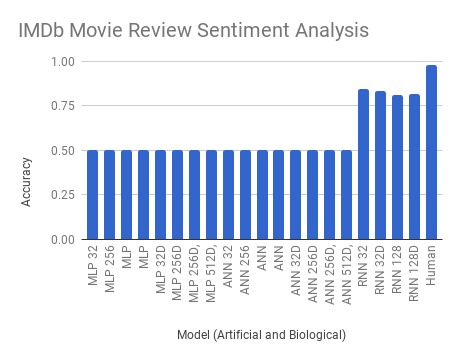
\includegraphics[width=\textwidth]{chart3.png}
	\end{subfigure}
	~
	\begin{subfigure}[b]{0.45\textwidth}
		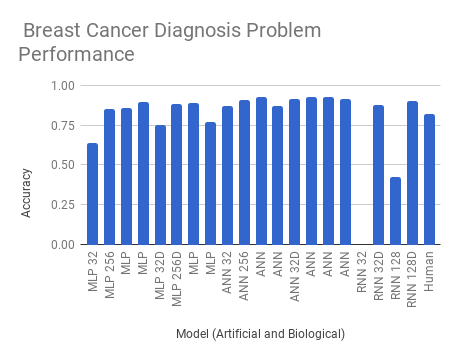
\includegraphics[width=\textwidth]{chart4.png}
	\end{subfigure}
	~
	\begin{subfigure}[b]{0.45\textwidth}
		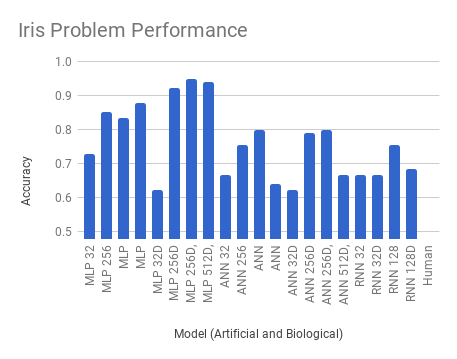
\includegraphics[width=\textwidth]{chart5.png}
	\end{subfigure}
\end{figure}


\section{Discussion}

The Recurrent Neural Networks performed best across all problem domains out of the artificial models. Of the RNNs, the most complex RNN with 1 hidden layer with 128 neurons and 20\% dropout performed the best, with an error standard deviation of 10.2\%, the lowest across all artificial models, and the third highest mean performance (1.11\% behind the \emph{MLP 256D}). The RNNs were heavily advantaged in the sentiment analysis problem, as they were the only models capable of creating meaningful feature relationships between the data and the expected results, as it was sequential. None of the other models converged on the sentiment analysis problem, as they recieved the data as a single contiguous stream without word boundaries, without any constant feature mapping for each step in the process of SGD optimisation that did not rely on sample memorisation, which would have led to extreme overfitting. As a result, the accuracy on the sentiment analysis problem for all MLP and ANN models was equivalent to random guesswork over the 25000 test reviews supplied to the program; such that the accuracy was $\frac{1}{|C|} = \frac{1}{2} = 0.5$ where $C$ is a set of valid output classes (in this instance a set of two classes --- positive and negative sentiment).

Despite RNNs having the advantage in the natural language parsing problem domain, RNNs did not have time to fully converge in the MNIST digit recognition problem. Even when MNIST images were downsampled to a ninth of the size specifically for the MNIST-RNN test combination, each of the 8 training epochs took an average of 20 minutes, as opposed to an average of 3.630 seconds in all of the ANN and MLP models. In fact, many of the more optimised ANN models (primarily those with 20\% dropout) began to diverge in under a minute, becoming overfit to the training data such that they lost accuracy on the test set. This is both due to the computational complexity of evaluating the data flow of an RNN relative to that of an ANN, and to the fact that there were thousands of times more trainable parameters subject to the stochastic gradient descent algorithm in RNNs as in the ANNs and MLPs (to illustrate, the simplest ANN had 59 trainable parameters, whereas the most complex RNN had 233223 trainable parameters). ANNs were much faster to train (in one test run, the \emph{MLP 512D,512D} achieved 99.41\% test accuracy after 3.640 seconds of training) and performed much better on non-sequential data, but entirely failed to converge on the sentiment analysis problem.

The higher-end MLP and ANN models with dropout (\emph{MLP 512D,512D} and \emph{ANN 512D,512D}) reached extremely high accuracy on the MNIST digit recognition problem; the ANN achieved 99.71\% accuracy, a mere 0.06\% behind the world record (\cite{ciregan2012multi}), despite being one of the simpler models and requiring under a minute to complete 20 training epochs, using hardware acceleration on a consumer-grade graphics processing unit.

There was one test which failed entirely --- the \emph{RNN 32} against the cancer diagnosis problem. For some unknown reason the network failed to learn from the data entirely and persistently resulted in an accuracy of 0, although the \emph{RNN 32D} which differed only in having 20\% dropout achieved 87.67\% accuracy on the same problem, and the \emph{RNN 128} achieved 42.25\%. This error is likely due to a problem with the primary dependency Keras (see \emph{Implementation Details} on page \pageref{sec:Appendix_I}) or the way in which the programs used interface with it, as the \emph{RNN 32D} and \emph{RNN 128} were both unaffected despite sharing the same code, aside from hyper-parameters specified at runtime.

\section{Conclusion}

Overall, it is clear that Recurrent Neural Networks are the future of machine learning. Even if they do not necessarily use the LSTM neuron model used in this experiment, the way in which they are able to interpret sequential data makes them much more valuable across differing problem domains. They are also much more closely modelled to the human brain, which is and has been the blueprint for machine learning models since the inception of the field late last century, and is the source of inspiration for many of the successful model architectures within the field, from simple binary perceptrons to LSTM neurons capable of drawing meaningful relationships in a series of sequential data.

However, overall the human brain performed the best in this experiment. Whilst many of the artificial models surpassed human ability in one or two problem domains, no single artificial model surpassed the human brain in every task, despite the tasks being relatively simple for a neural network to solve (with the exception of the sentiment analysis problem). Despite having less training time, the human brain was still the most neuroplastic.

All in all, this experiment has shown that state-of-the-art artificial intelligence techniques, despite having superhuman results in very narrow problem domains, are far from achieving general intelligence, at least given current hardware. The human brain still has 7 orders of magnitude more neurons than the most expansive of the models utilised in this experiment (1024 neurons compared to approximately 100 billion (\cite{herculano2009human})), and has mechanisms at play so complex that researchers have struggled even to fully simulate the brain of the C.Elegans, a transparent worm with only 959 neurons, whose connectome has been fully mapped for decades (\cite{wormwiring2012}). At the current point in time, neither the software to supervise the training of an AGI nor the hardware to implement the data flow of the network (let alone the training, which is several orders of magnitude more computationally expensive) exists, and will not for many decades at the current rate of progress.

\begin{enumerate}
	\item Sigmoid, ReLU, heaviside
	\item Fix method, make reproducible, mention variables
	\item Human data
	\item Rubric
	\item Fix (!)s
	\item Tables?
	\item Charts
	\item Use neuroplasticity as a training target? Train hyper-parameters?
	\item Fonts
\end{enumerate}

\section{Appendices}

\label{sec:Appendix_I}
\subsection{Appendix I: Implementation Details}

All of the deep learning models tested were implemented in the Python 3 programming language, using the Keras machine learning library with a TensorFlow backend. It was decided to use a stable machine learning framework such as Keras to create easily reproducible results and to make it much easier to verify that the programs used in the experiment do not have any flaws undermining their validity.

The Python 3 source code files for all of the aforementioned artificial models are available online through the Git repository hosted at following URL: \texttt{https://github.com/Tobsta/ScienceFair/tree/master/src}. Each overarching model architecture (ANN, MLP, RNN) has its own file (\texttt{src/ann.py} etc.) which accepts a loaded dataset and hyper-parameters from the main program, and each dataset has its own file which serves to load it from memory. The main program which coordinates the interaction between the models and the datasets is in the file \texttt{src/main.py}, which can be run in a terminal using the command \texttt{python3 main.py}. The program's dependencies include Tensorflow (\texttt{tensorflow-gpu==1.5.0} used in testing), Keras, and numpy; all of which may be installed using Python's \texttt{pip} package manager.

\twocolumn
\label{sec:Glossary}
\subsection{Glossary}
\begin{description}
\item[Activation function:] A function used to transform the output value of neurons to adapt the rate at which they learn. Examples include the sigmoid and ReLU functions.

\item[Artificial General Intelligence (AGI):] An intelligent agent capable of learning to accomplish many general tasks at least as well as a human, as opposed to specialising in a particular task. At this stage, AGIs are mostly a topic of science fiction and radical speculation; however many experts believe that general intelligence is mere decades away. In a survey of prominent AI researchers, the median estimation for when there will be a 50\% chance of AGIs having been developed was 100 years from 2016 (\cite{grace2017will}).

\item[Artificial Neural Network (ANN):] An interconnected network of artificial (simulated) neurons that receive signals (in the form of binary or floating point numbers) as input, which pass through the connections between nodes in the network toward the output layer of neurons which emits a computed result. Simple ANNs typically contain an input layer, one or more hidden layers for complex computation and feature mapping, and an output layer.

\item[Classification problem:] A type of machine learning problem in which a series of data is labelled according to a few predefined classes. Examples include Optical Character Recognition and Computer Vision problems; the most common of which is handwritten digit recognition.

\item[Convolutional Neural Network (CNN):] A neural network in which some layers are not composed of artificial perceptrons, but instead of convolutional kernels that operate over a multidimensional space transforming each value by an operation configurable in training. CNNs are often used for image feature extraction.

\item[Cost function:] A function that estimates the accuracy/error rate of a model; lower is better.

\item[Dropout:] A technique to avoid overfitting in ANNs. It works by randomly removing a constant percentage (configurable as a hyper-parameter, 20\% in this experiment) of nodes from a hidden layer in a neural network (\cite{dropout14}), which reduces overfitting and makes computations by a model more generalised, with the additional benefit of making the model less computationally expensive to operate further into the training process.

\item[Feed-Forward ANN:] A class of ANN which has distinct layers of neurons whose signals are only fed forward. This significantly reduces the complexity of neural networks, and means that the neural network is not capable of retaining information (unlike an RNN).

\item[Hidden Layer:] A layer of artificial neurons that does not directly deal with input or output, but instead performs highly complex logic derived from model permutations tested in training.

\item[Hyper-parameter:] A global parameter in an artificial model that is pre-selected by the model designer and which dictates how the model will be organised or how it will train. The number of neurons in a hidden layer and the learning rate (step size of the SGD algorithm) are both examples of hyper-parameters.

\item[Input Layer:] A layer which does not take input from the previous layer, but rather from the host program, usually in the form of a sample in a dataset specific to the problem domain the model is being trained for.

\item[Learning function:] See \textit{Activation Function}

\item[Learning rate:] A hyper-parameter that is used as the maximum deviance random permutations made during the process of stochastic gradient descent may be. A higher learning rate means the model will train faster and will not fall into any local minimums, but also means it may not converge as well, unless the learning rate is decreased each epoch to make it more sensitive to fine-tuning.

\item[Long Short-Term Memory (LSTM):] A type of artificial neuron used in RNNs, designed to retain information for sequential information processing.

\item[Machine Learning:] A subfield of artificial intelligence that deals with teaching machines to learn, specifically through pattern recognition, feature-mapping, evolutionary algorithms, and inference engines.

\item[Neuroplasticity:] The ability of a brain or machine learning model to adapt to fit different problem domains without modifying the overall structure (i.e. by changing only the synapse connections and activation thresholds for neurons, and not the underlying algorithms).

\item[One-Hot Encoding:] The process of converting a class label to an array of numbers equal to the number of classes, populated with zeros, aside from the number at the index of the class label, which is a one. To illustrate, the classes "Cat", "Dog", and "Horse" could be represented as [1,0,0], [0,1,0], and [0,0,1] with one-hot encoding assuming the full ordered set of classes is {"Cat", "Dog", "Horse"}. One-hot encoding is better than other encoding methods for feature mapping algorithms operating on classed data, especially in an output layer of a classification model (see \emph{softmax}).

\item[Output Layer:] The layer which creates the final computation and returns it to the host program. In classification problems, each neuron in the output layer will typically map to a class in the dataset. The result of the output layer is then compared to the one-hot encoded class of the sample in the cost function to determine the error rate.

\item[Overfitting:] The process of over-training a model; an overfit model is so finely tuned to its training dataset that it performs poorly during validation and testing.

\item[Perceptron:] A common, but outdated, artificial model of a neuron which has a binary as opposed to floating-point output. This means as a small change in inputs creates a much larger change in output, they are much less sensitive to training algorithms such as SGD.

\item[Recurrent Neural Network (RNN):] A neural network which runs recursively on a sequence of data, using previous inferences as input in addition to the next segment of data. RNNs are predominantly used for speech recognition, text classification (such as sentiment analysis) and many other problem domains in which the data is sequential and the length is variable; although RNNs can also be trained to work as less efficient ANNs with fixed vector size inputs and outputs.

\item[Regression problem:] A type of problem where a model is trained to find the relationship between input and output data. One example of a regression problem is estimating the selling price of a house given data on it (such as the number of bedrooms).	

\item[ReLU (Rectified Linear Unit)] A simple activation (learning) function that returns the greater out of the input or 0.

\item[RMSprop] A learning algorithm (not to be confused with a learning/activation function) similar to SGD, except the learning rate is adjusted given the gradient of each trainable parameter of the model, instead of being specified as a hyper-parameter. This means that the model is robust against both falling into a local minimum and plateauing during training, and to being so insensitive to a steep gradient that it diverges away from the global minimum.

\item[Sigmoid function:] A learning function that creates an S-shaped curve with a steeper gradient toward the middle. It is used to force parameters to either extreme, speeding up the early stages of training.

\label{itm:SGD}
\item[Stochastic Gradient Descent (SGD):] A method of minimising the error function of a neural network model (or other machine learning model) given multivariate input, in which the the input parameters are viewed as axes on an n-dimensional graph with the cost (error) function as the Y-axis. SGD attempts to find the global minimum of the cost function without calculating it for every possible combination of parameters by 'rolling a ball down a hill'; where the ball is a vector representing the weights and biases of the neural network in the latent space, and the hill is the aforementioned n-dimensional graph. In each iteration of the SGD algorithm, the direction gradient toward the local minimum is estimated by calculating the partial derivative of the cost function with respect to each parameter, and determining which parameter, plus-minus the learning rate hyper-parameter, has the lowest resultant cost function value. The relevant parameter is then shifted to the new position. Typically, there will be millions of iterations.

\item[Softmax:] An activation function that scales all outputs from a layer from 0 to 1, such that the sum of all outputs is 1. It is typically used for the output layer of a classification neural network, as a floating-point alternative to the one-hot encoding method.

\item[Support Vector Machine (SVM):] An older algorithm machine learning which uses a mathematically and not biologically inspired linear and non-linear regression algorithms to classify data.
\end{description}
\onecolumn

\printbibliography

\end{document}          
